\chapter{Future work}\label{chapter:future-work}

This master thesis was primarily focused on implementing a prototypical micro-frontend architecture to replace AGnet's internal \ac{ERP} sytem sometime in the future. The work examined whether using GraphQL with Apollo Client can bring performance improvements inside a micro-frontend architecture. The improvements with GraphQL were implemented with two methods. First, a caching layer was shared across all micro-frontends. Second, the GraphQL Client layer should remove fields from queries that are already stored within the cache. Using a single cache instance for all micro-frontends has led to significant improvements regarding request size and response size. The second method of improving performance by reducing the fields of a query was auspicious, but it did not produce significant improvements in the prototype scenario. The screen design and structure of the prototype follow the approach of a list view, showing a table with some fields. In addition, a detail view for each table row view mainly loads all the fields in the object; however, the table view does not prefetch and cache enough fields to make a difference in query and response size. However, other applications with a different design could benefit from reducing queries with existing data. The following section explains a theoretical example of an application that could benefit from reducing queries.

\subsubsection{Example of an e-commerce platform benefiting from query reduction and a shared cache layer}

This section describes a fictional application that could improve significantly using query reduction and a shared caching layer. The application is an e-commerce platform, which has the same architecture as the micro-frontend prototype. The e-commerce application contains multiple micro-frontends, each responsible for a different part of the shopping experience. The micro-frontends for an e-commerce application could include multiple widgets on the landing page, product browsing, product detail, shopping cart, checkout process, and order tracking. A possible journey through an e-commerce application is shown in Figure \ref{fig:future-work:flow-chart}.

\ifshowImages
\begin{figure}[H]
  \centering
  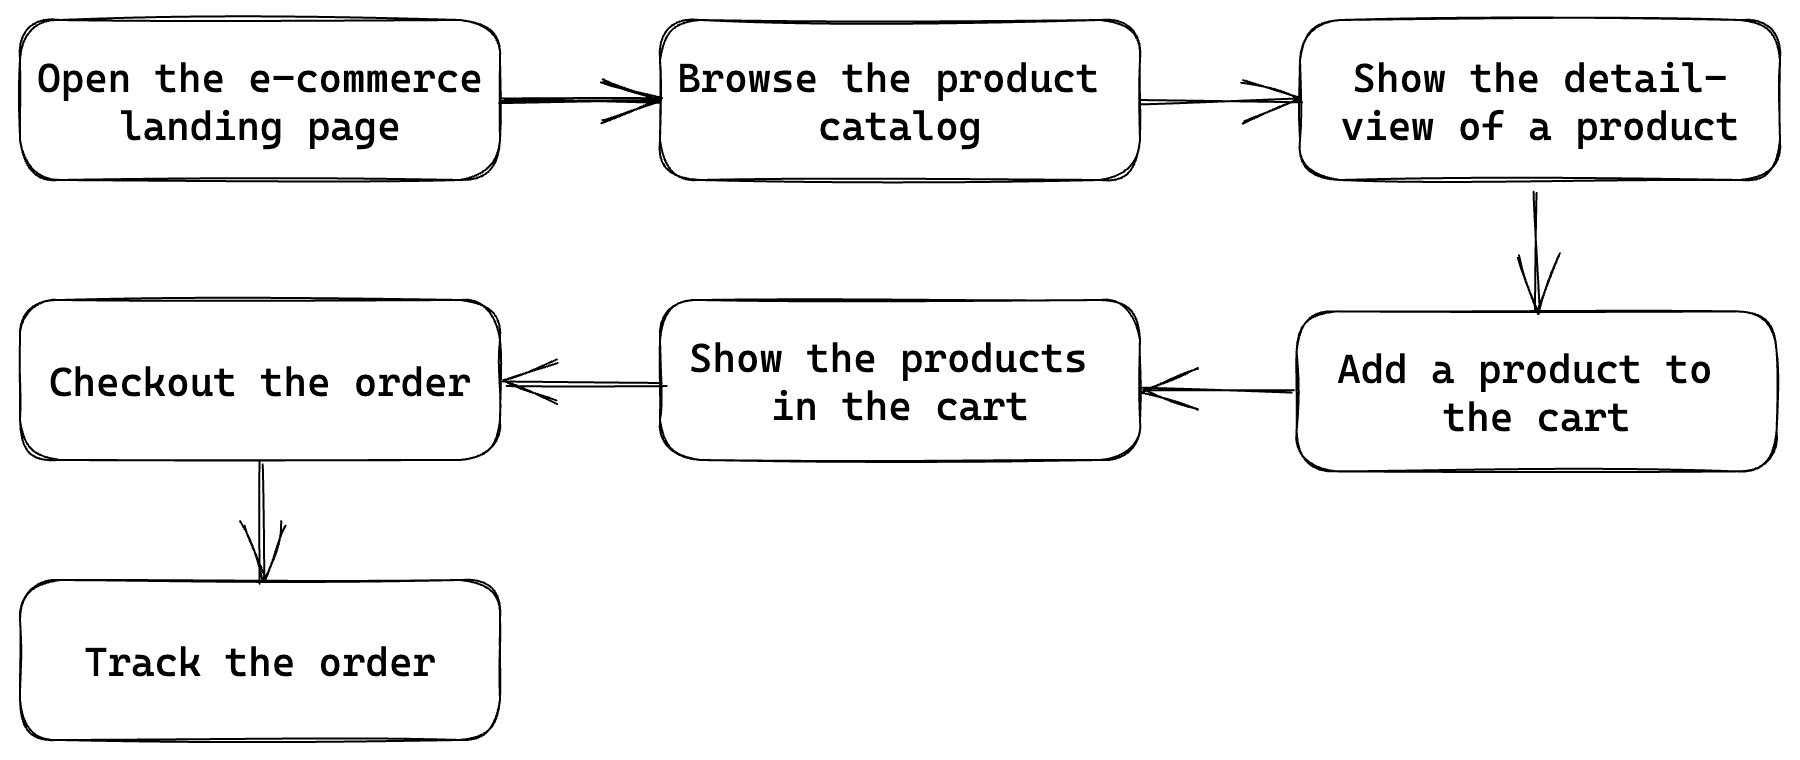
\includegraphics[width=0.8\linewidth]{images/future-work/flow-chart-e-commerce.png}
  \caption{A possible user journey through an e-commerce application.}\label{fig:future-work:flow-chart}
\end{figure}
\fi

\noindent The user first opens the landing page of the e-commerce platform. There he sees a list of recommended products and a list of product categories. The images and some information about the suggested products are loaded and stored in the cache. The user clicks on a recommended category and is redirected to the product browsing micro-frontend. The product browsing page displays a list of products in the selected category. The first products shown in the category are the same as on the landing page. Therefore, some data, including the product name, user rating, price, and image, can be reused from the cache. If the user scrolls down, the missing products are loaded from the server, rendered to the screen, and stored in the cache. Once the user finds a product they like, they can view the detail view. The detail view shows the product name, images, price, description, user rating, and reviews of other users. Much of the more important data, such as the product images displayed on the page, can be reused from the cache, allowing the page to render faster. Once the user has found a product he wants to order, he can add it to the shopping cart. When the user is ready to purchase the items in his shopping cart, he proceeds to the checkout. At the checkout, the user's address, the selected products and the total price are displayed. The information about the products can be completely reused from the cache. The information about the user's address can be reused from the cache. They enter their shipping and billing information, choose a payment method, and verify their order information. After submitting the order, the user receives a confirmation page with the order number, the ordered products and the expected delivery date. The user can track the status of his order and the progress of delivery. This information can also be fully reused from the cache if it is the same session.

\bigskip

\noindent This type of application benefits greatly from the shared caching layer and the mechanism for removing fields from a query that are already in the cache. The products are the main citizens of the e-commerce application. The shared caching layer is as important as it is in the micro-frontend prototype and allows most of the information to be reused. The user sees the same products on the landing page, product overview page, product detail page, shopping cart, checkout process, and order summary. So the product data is cached and can be used and extended on each page, which also benefits the subsequent pages.

\subsubsection{Further prototype development}

The current focus is on the further development of the micro-frontend architecture. The prototypical implementation carried out in this master thesis has only implemented a small subset of the functional requirements of the overall system. However, the basic structure that all micro-frontends must follow was defined and easily accessible. The process of creating, integrating, and configuring a new micro-frontend is also clearly defined and follows a standardized principle. The steps tp create, configure, and add a new micro-frontend to the architecture could be automated in the future using Angular's Schematics\footnote{\url{https://angular.io/guide/schematics}}.
